%%%Estructura:
%Introducción al problema de conteo de personas + como vamos a juntar IA+Estereologia.
%Introducción a la estereología (Historia/Intro + Test system que usamos + limitaciones de la estereología [conteo tiene que ser manual])
%Introducción a la IA/Machine Learning (Historia/Intro + que usamos + tabla de modelos de conteo de personas actuales)
%%%%%%%%%%%%%%%%%%%%%%%%%%%%%%%%%%%%%%%%%%%%%%%%%%%%%%%%%%%%%%%%%%%%%%%%%%%%%%%%%%%%%%%%%%%%%%%%%%%%%%%%%%%%%%%%%%%%%%%%%%%%%%%%%%%%%%%%%%%%%%%%%%%%%%%%%%%%%%%%%%%%%%%%%%%%%%%%%%%%%%%%%%%%%%%%%%%%%%%%%%%%%%%%%%%%%%%%%%%%%%%%%%%%%%%%%%%%%%%%%%%%%%%%%%%%%%%%%%
%%%%%%%%%%%%%%%%%%%%%%%%%%%%%%%%%%%%%%%%%%%%%%%%%%%%%%%%%%%%%%%%%%%%%%%%%%%%%%%%%%%%%%
%%INTRODUCCION
This master's final project focuses a specific field of Artificial Intelligence (AI), crowd counting. However, the basis on which our estimation method is based involves a specific field of mathematics, Stereology. Even though we tested our method's performance in crowd counting, the methodology used for this project can be adapted so as to be employed in a similar manner for many different problems.\\

Crowd counting revolves around the estimation of the number of individuals in images or videos. Because of its potential applications in critical areas, such as managing pandemics, averting crowd collapses, enhancing public safety, urban planning and event management, this task has garnered considerable attention in recent years. When it comes to AI, the objective is to automatically estimate the number of individuals, without involving human interaction in the counting process. As humans, we can accurately determine if we are seeing a person in an image, so counting people is easy, but a laborious and time consuming job. 
%%DomingoMaster: En vez de AI, however,. Lo he hecho asi porque creo que se entiende mejor, humanos <-> computadores
In contrast, a computer can count in a very fast manner, but it needs to be ``trained'' in order to accurately count people in images, and even then, its performance may be pitiful depending on the underlying structure of the training algorithm. \cite{CLIP} is among the state of the art for this field. \\

In a previous work~\citep{TFG}, we combined some Stereology based methods with the potential of computers in order to see the performance improvements and the accuracy of these methods as opposed to straightforward computer calculations with regards to point counting and length estimation. Here, we take a step forward and use our former work to show how AI and Stereology can be combined so as to achieve better performance and accurate results.

%???????????????????????????????????????????


%%%%%%%%%%%%%%%%%%%%%%%%%%%%%%%%%%%%%%%%%%%%%%%%%%%%%%%%%%%%%%%%%%%%%%%%%%%%%%%%%%%%%%
%%ESTEREOLOGIA
\section{Stereology}
%INTRO
A general problem is to estimate a quantity from an object, relaying only in a finite number of samples and the method used to acquire them.
%Texto de introducción sobre el uso de la estereología actualmente
When it comes to object sampling Stereology is the quintessential science, since it makes it able to estimate quantitative properties of spatial objects. According to \cite{CO.IAS.17.Hist.pdf}, ``Stereology is the science of geometric sampling'' whose applications extend to disciplines such as biology and materials science.\\

In traditional sampling on discrete populations, sampling units had to be accessible to observation. However, the target object in geometric sampling is a subset of space and the sample is obtained via the intersection between the object and what's called a \textit{test probe}. A \textit{test probe} is basically a regular arrangement of test points, lines, planes, or slabs whose size and shape are known and has some sort of randomness mechanism relative to the object (see \cite{CO.IAS.17.Hist.pdf}).\\

%PROBLEMAS
Because of Stereology requiring to ``manually measure'' what's needed to estimate those quantities its applications were scarce. However, as a result of computing and artificial intelligence being improved, we can now make use of Stereology procedures with little to no effort.\\

%DOMINGO

%Domingo: Dependiendo del tiempo que tengamos, quizás deberiamos poner algo de la estructura del documento.

This document is written with the aim to be accessible to all people, but the in depths behind the theory may be easily understood for people with a degree in mathematics and/or data science/artificial intelligence. Although this work tries to be self-contained, some results and concepts like dimension, measure, etc. are not formally defined inside the document and we operate with them in an intuitive fashion.\\

\textit{Remark.} During Chapters \ref{cap:Intro} and \ref{cap:Teoria}, a lot of history, theory and results have been gathered together in order to provide a simple understanding of the procedure and lead towards what we want to accomplish in this work. Therefore, the structure and information from these chapters will resemble to the ones from \cite{CO.IAS.17.Hist.pdf}, \cite{SterThAppl-2022-07-21.pdf}, \cite{Leobacher_Pillichshammer___2013___Introduction_to_Quasi_Montecarlo_Methods.pdf} and \cite{Hinrichs.pdf}.\\

\subsection{History of Stereology}
%%%%%%%%%%%%%%%%%%%%%%%%%%% PROBLEMA: la historia está bastante copiada del pdf

%%%%%%%Historia
The underlying theory of Stereology is a blend of integral geometry, probability and statistics expected to be used in biomedical and material sciences. Since its development was focused on these two disciplines, Stereology can be divided in two branches depending on the application: 
%Domingo
\begin{itemize}
    \item \textit{Design based Stereology}: this area does not make any assumption about the data and the inference process is based on the randomness of the samples. It is more centered on biomedical applications, thus the object is assumed to be fixed and bounded and sampling is done with randomized test probes.
    \item \textit{Model based Stereology}: in this area there are some assumptions about the samples, specially some homogeneity in the object is assumed. It is more centered on material science applications where the object is huge, thus dealing with small portions of practically unbounded spacial structures and randomness being incorporated by means of a random set model (relies on model shapes, thereby usually leads to biased methods).
\end{itemize}
%DOMINGO.
Another distinction can be done regarding stereology that splits it into \textit{global stereology} and \textit{particle stereology}:
\begin{itemize}
    \item \textit{Global stereology}: In the design context it deals with total quantities (\textit{e.g.} total number, length, area, volume...). In the model context it deals with ratios (\textit{e.g.} relative volume).
    \item \textit{Particle stereology}: It deals with mean properties of individual particles (\textit{e.g.} mean volume).
\end{itemize}

Just as an introduction to this science, let's consider an equivalent problem to Buffon's needle problem, which is said to encapsulate the art and spirit of Stereology:\\
%Domingo
\begin{tcolorbox}
A needle of length $\ell$ is arbitrarily fixed inside a disk of diameter $h > \ell$ in the plane. A straight line in the same plane hits the disk at random. Calculate the probability that the straight line hits the needle\\
\end{tcolorbox}
%DOMINGO
Buffon's problem incorporates both a uniform random location of the center of the needle and a uniform random orientation (isotropic orientation) of the needle. We sketch the proof for the close formula for this probability using simple arguments. 
%Domingo: Aqui se hablaba de varias lineas pero en el  problema de buffon de una sola. He añadido una explicacion
An experimental approach would be to place ``random lines'' and count the proportion to estimate the probability.  
Now, if the number of random lines that hit the needle and the number of lines that miss the needle are known, then the ratio of those numbers would solve the problem. However, here it is necessary to use some sort of continuous geometric measure rather than traditional counting.\\

The following is a sketch with the main ideas needed to find the solution to Buffon's problem.
Let $L_1^2$ be a straight line used as a \textit{test probe}. This straight line can be defined with two coordinates $(p,\phi)$ in the plane, where $p \in (-\infty,\infty)$ is the distance of the line from a fixed origin $O$, and $\phi \in [0,\pi)$ is the orientation angle. Furthermore, the line can be associated with a density $\mathrm{d}L_1^2=\mathrm{d}p\mathrm{d}\phi$. Using this density, the total number of all straight lines hitting a convex set of boundary length $B$, is exactly $B$.\\
%DOMINGO (Quiza una referencia a la densidad y donde está el resultado con la página del libro de Luis)

%Domingo
For a needle of length $\ell$, the hitting measure (namely the measure of all the probes hitting the set) is $2\ell$. The reason is because the needle has to be regarded as a flattened convex set of perimeter $2\ell$. For the same reason, the hitting measure is $\pi h$ for a disk of diameter $h$. Therefore, the probability is $2\ell/(\pi h)$.\\
%DOMINGO


This result aroused controversy, %Domingo: Referencia? 
resulting on the appearance of paradoxes such as ``Bertrand's paradoxes''. A few years later it was discovered that measure densities had to be motion invariant, %Domingo: Referencia?  (Co.hist, está abajo)
that is, invariant with respect to translations and rotations, therefor making them independent of the reference frame.\\

All these events made integral geometry emerge as a mathematical discipline used to obtain motion invariant densities for geometric objects, thus establishing a foundation of geometrical probability. Some typical integral geometry results are the Crofton formulas, which relate intersections between two objects and their properties (number, length, area, volume...). %Domingo:REferencia (Co.Hist) y explica que son en una frase y porque son interesantes para nosotros (solo se usan para la explicación de como se obtiene un estimador en estereología)
For example, let $Y$ be a bounded planar curve  of finite length $B$. The measure of the number $I(Y\cap L_1^2)$ of intersections determined by all the motion invariant straight lines hitting the curve is 
\begin{equation} \label{eq2}
    \int_{Y}  I(Y\cap L_1^2)\,\mathrm{d}L_1^2 = 2B
\end{equation}
%Domingo: Me costo entender que tenia en este parrafo.
If $Y$ is the boundary of a convex set, then $I(Y\cap L_1^2)=2$, therefore the preceding formula yields the solution of Buffon's problem, noting the hitting measure is $B$.\\

%Domingo: He escrito esta frase, pero no sé que te parece
The minimal requirement to sample by intersecting with a probe is that we obtain information. For that,
Stereology also takes into account dimensional considerations in order to obtain the desired quantity. Depending on the dimension of the object and the probe, different procedures can be used and
%Domingo: he cambiado measures por parameters
different parameters have to be taken into account. To be more specific, for an object $Y$ hit by a probe $T$ in $\mathbb{R}^d$,
\begin{equation*}
    dim(Y\cap T) = dim(Y) + dim(T) - d
\end{equation*} 
holds up to a set of positions of zero measure. Since $dim(Y\cap T)\geq 0$, the following inequality must always hold,
\begin{equation}\label{eq1}
    dim(Y) + dim(T)\geq d.
\end{equation} 

%Domingo: Siempre que pongamos referencia a una formula, ponemos eqref
If equation \eqref{eq1} holds and either $dim(Y)=d$ or $dim(T)=d$, then relating $Y$ and $T$ by a Crofton formula is viable as long as $T$ has a fixed orientation relative to $Y$. On the other hand, if $dim(Y)<d$ and $dim(T)<d$, then the density of $T$ has to be motion invariant.\\

%Domingo: No sé si hace falta una frase para unir el parrafo anterior con este. (está en orden cronológico)
The next breakthrough in history was that Buffon's problem and the development of sampling and statistics in the 20th century inspired estimation problems. Furthermore, proper probability measures for random probes were defined, which was fundamental in the development of Stereology. For instance, the probability element associated with a test line hitting a disk is $$ \mathbb{P}(\mathrm{d}p,\mathrm{d}\phi) = \frac{\mathrm{d}p\mathrm{d}\phi}{h\pi}, \hspace{2mm} p\in[-h/2,h/2], \hspace{2mm} \phi \in [0,\pi), $$
namely the motion invariant density normalized by the measure of all test lines hitting the disk. This probability element implies that $\phi \in [0,\pi)$ is \textit{uniform random} (UR), that is, \textit{isotropic random} (IR) in the unit semicircle, whereas $p \in [-h/2,h/2]$ is independent and UR. Therefore, the test line is said to be \textit{isotropic uniform random} (IUR) hitting the disk.\\

%Domingo: No es tanto un ejemplo como una aplicacion a un problema. Hay que leerse este parrafo.
To show an application of the formula in equation \eqref{eq1} to an estimation problem, suppose $Y$ is a planar curve with unknown length $B$ contained in a disk of diameter $h$.  
We suppose that the curve is not possible to manipulate (straighten the curve, cut into pieces, etc) and it is necessary to estimate the parameter $B$.
In order to do that, we design the following sampling experiment or estimator.
The sampling experiment consists of a disk being hit by a IUR test line $L_1^2$. Considering equation \eqref{eq2}, since $I(Y\cap L_1^2)$ is an integer valued random variable, its expectation (mean value) is $$ \mathbb{E}[I(Y\cap L_1^2)] = \int  I(Y\cap L_1^2)\,\mathbb{P}(dp,d\phi) = \frac{2B}{h\pi}. $$
Therefore, $\widehat{B}=\frac{h\pi}{2} \cdot I(Y\cap L_1^2)$ is an \textit{unbiased estimator} (UE) of $B$.\\

%Domingo: He cambiado algo
On one hand, the mean of different unbiased estimations taken at random and independently can be used to approximate the length better.
On the other hand, one inconvenience of the following estimator is that some of those estimations could give wrong results, e.g. certain estimations can be zero if the test line misses the curve, which results on time and effort spent uselessly. 
%Domingo: He tenido que añadir que es systematic sampling and 
In practice, \textit{estimators} which sample in a strategic way, v.g. adding more test lines, is more convenient and generally more efficient than independent sampling because estimations are rarely zero and variances tend to be significantly lower (see \cite{CO.IAS.17.Hist.pdf}).\\

These gives two basic strategies for sampling:
\begin{itemize}
    \item Random sampling: which estimates the measures using different results obtained for random test probes.
    \item Systematic sampling:  which estimates the measures using specific test probes that may get better results. This usually implies some kind of dependence between samples.
\end{itemize}
%%%%%%%%%%%%%%%%%%%%%%%%%%%%%%%%%%%%%%%%%%%%%%%
%TEST SYSTEM
\subsection{Estimation Problem. Test System of Quadrats}
%%%%%%%%%%% Buffon y conteo
Now that some of the basic concepts and ideas about Stereology have been introduced, lets focus on the estimation problem that will be used for our estimation method.\\
\textbf{Notation}: 
Through the rest of the thesis, we use the following conventions,
\begin{enumerate}
    \item $Y$ will denote a compact set with $dim(Y)=q$ and \textit{q}-measure $\gamma(Y)$. For example, if $Y\subset \mathbb{R}^3$, then $\gamma(Y)$ may represent number of subsets, curve length, surface area or volume, depending on whether $q=0,1,2,3$ respectively.
    \item $L_r\equiv L_r^d, \hspace{2mm} r=0,1,...,d$ will denote an \textit{r}-plane in $\mathbb{R}^d$, for instance, a test point, line, plane or slab according to whether $r=0,1,2,3$ respectively.
    \item $\alpha(X)$ will denote the geometric measure of a compact set $X$, thus $\alpha(\emptyset)=0$. For example, if $Y\subset \mathbb{R}^3$, then $\alpha(Y\cap L_r)$ will represent number, length, area or volume, depending on whether $q+r-d=0,1,2,3$, respectively.
\end{enumerate}

%Domingo :  Maybe to add a phrase about what is a test quadrat of area. Maybe a graph.
Suppose $Y=\{ y_1,y_2,...,y_N \}\subset D \subset \mathbb{R}^2$ is a finite set of $N$ disjoint point particles where $y_i$ denotes the \textit{i}-th point particle and $D$ is a reference disk of diameter $H$. Consider $T_2^2(x,\omega)$, a test quadrat (square) of area $a$ and random fixed orientation $\omega \in [0,2\pi)$ that's free to move parallel to itself with translation invariant density $dT_2^2(x,\omega)=dx$. We have
\begin{multline} \label{eq3}
    \int_{\mathbb{R}^2}  N(Y\cap T_2^2(x,\omega))\,\mathrm{d}x = \int_{\mathbb{R}^2} \sum_{i=1}^N 1_{T_2^2(x,\omega)}(y_i),dx = \int_{\mathbb{R}^2} \sum_{i=1}^N 1_{T_2^2(0,\omega)}(y_i-x),dx \\ = \sum_{i=1}^N \int_{\mathbb{R}^2}  1_{T_2^2(0,\omega)}(y_i-x),dx = Na 
\end{multline}

The probability element for a quadrat with fixed orientation $T_2^2(x)$ hitting a disk $D$ is
\begin{equation*}
    \mathbb{P}(dx)=\frac{dx}{A(D_{\oplus})}, \hspace{2mm} x\in D_{\oplus}.
\end{equation*}
where $A(D_{\oplus})$ is the area of the geometric loci of the AP as the test probe hits D. Therefore, the number of point particles is
\begin{equation*}
    N=\frac{A(D_{\oplus})}{a}\cdot\mathbb{E}(Q(x))
\end{equation*}
where $Q(x)$ is the number of point particles captured by the quadrat. Similar results can be obtained for $\mathbb{R}^d$.\\

Since the quadrat's orientation is fixed, it is usually called a \textit{FUR quadrat} (Fixed Uniform Random). Let's consider a FUR quadrat $T_0 \equiv T_2^2(0,\omega) \subset J_0 \subset \mathbb{R}^2$ of area $a_0 > 0$ and fixed orientation $\omega \in \mathbb{S}$ where $T_0$ is what's called a \textit{fundamental probe} contained in a \textit{fundamental tile} $J_0$ of the test system. A \textit{FUR test system of quadrats} can be defined as 
\begin{equation*}
    \Lambda_x := \{ T_2^2(x+t_k,\omega), k\in \mathbb{Z} \}, \hspace{2mm} x \sim UR(J_0)
\end{equation*}
% Domingo: Aquí haria falta una referencia a la página (229 pdf).
Considering equation \eqref{eq3} and Santaló's formula for FUR test systems with bounded fundamental test probes $T_0\subset J_0\subset \mathbb{R}^d$,
\begin{equation*}
    \gamma(Y)\nu(T_0)=\int_{J_0}  \alpha(Y\cap \Lambda_x)\,\mathrm{d}x
\end{equation*}
where $\gamma(Y)$ is the target measure, $\nu(T_0)$ is the known measure for the fundamental probe and $\alpha(Y\cap \Lambda_x)$ is the geometric measure of $Y\cap \Lambda_x$, we have
\begin{equation*}
    \gamma(Y)\cdot a_0 = \int_{J_0}  \alpha(Y\cap \Lambda_x)\,\mathrm{d}x = a\cdot \mathbb{E}[\alpha(Y\cap \Lambda_x)]
\end{equation*}
where $a\geq a_0$ is the area of $J_0$. Therefore, the basic identity for a FUR test system of quadrats is
\begin{equation} \label{conteo}
    \gamma(Y)=\frac{a}{a_0}\cdot \mathbb{E}[\alpha(Y\cap \Lambda_x)]
\end{equation}
where $\gamma = N \text{ (number)},B \text{ (length)},A \text{ (area)}$ depending on whether $dim(Y)=0,1,2$ respectively (\cite{SterThAppl-2022-07-21.pdf}).\\

In this work, $Y$ will be a set of people's head centers (assumed as the point particles in the estimation problem) representing people in different images. This means that $dim(Y)=0$, thus the identity that will be used reads
\begin{equation} \label{Conteo_usada}
    N =\frac{a}{a_0}\cdot \mathbb{E}[N(Y\cap \Lambda_x)]
\end{equation}

Later in this work we will use the aforementioned identity to estimate the amount of people present in images and compare the efficiency of several AI crowd counting methods with our method, which will be explained later.\\




%
%
%
%
%
%
%
%
%
%
%
%
%
%
%
%
%
%
%
%
%
%
%
%
%
%
%
%
%
%
%
%
%%%%%%%%%%%%%%%%%%%%%%%%%%%%%%%%%%%%%%%%%%%%%%%%%%%%%%%%%%%%%%%%%%%%%%%%%%%%%%%%%%%%%%%%MACHINE LEARNING
\section{Artificial Intelligence (AI)}
%INTRO
Artificial Intelligence is a discipline that encompasses several different processes concerned with making machines smart, aiming to create a system that behaves like a human. Machine Learning is a subset of Artificial Intelligence related with the study, design and development of algorithms that give computers the capability to learn without being explicitly programmed. Going even deeper in this discipline we have Deep Learning, a subset of Machine Learning in which data is passed via multiple non-linear transformations to calculate an output, where Artificial Neural Networks, also called Neural Networks (NN)\footnote{(\url{https://www.kdnuggets.com/2020/11/data-science-history-overview.html})}, reside. A Neural Network is a system composed of many simple processing elements operating in parallel whose function is determined by network structure, connection strengths and the processing performed at computing elements or nodes. They have a natural propensity for storing experiential knowledge and making it available for use, resembling the brain in two aspects: knowledge is acquired through a learning process; and neuron (node) weights are used to store the knowledge
(\cite{DARPA}, \cite{Haykin}). %pdf Intro ML1
As a result, it is said that Neural Networks are inspired in the structure and functioning of the brain, which is a collection of interconnected neurons:
\begin{itemize}
    \item Each neuron (node) consists of a cell body that contains a cell nucleus (activation function).
    \item Neurons have fibers, called dendrites, and a single long fiber, called axon, branching out from the cell body.
    \item The axon connects one neuron to others through the dendrites.
    \item The connection junction is called synapse.
    \item The synapse releases chemical transmitter substances (linear combination of nodes and node weights, plus a bias), entering the dendrite (node receives information), raising or lowering the electrical potential of the body.
    \item When the potential reaches a threshold (information passed completely), an electric pulse is sent down the axon (activation function applies) affecting other neurons (continue process with new nodes). 
\end{itemize} %Intro ML1
When a Neural Network uses this simple representation of biological neurons we say that nodes follow the perceptron model.\\

This analogy was used to interpret Neural Networks as a system of consecutive layers of nodes, with nodes in the first layer connected to nodes in the second layer and so forth. Typically, one talks about a Neural Network with one input layer (first layer), one output layer (last layer) and a certain amount of hidden layers, $n$ ($n$ layers in between). The input layer receives the "raw" information (even though it may have been preprocessed before training) and transmits it to the hidden layers. The hidden layers make use of the information and try to give the best results. Finally, the output layer interprets the results and gives an output in a specific format. 

\begin{figure}[h!]
  \begin{center}
    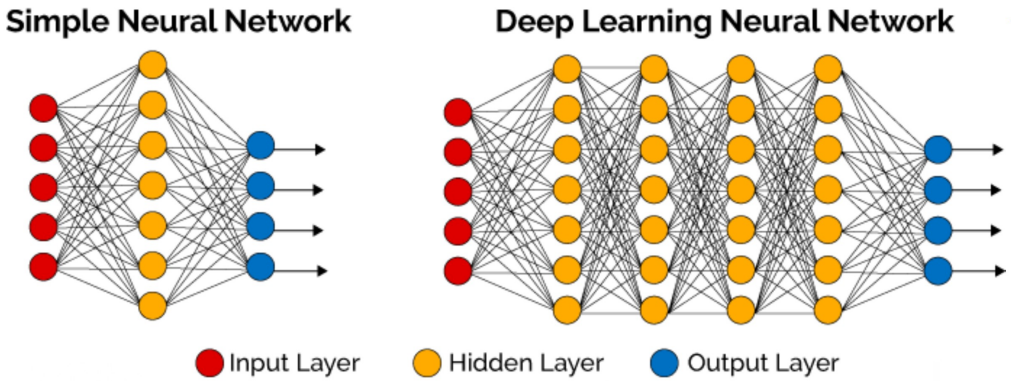
\includegraphics[width=120mm, height=45mm]{Figuras/NNgenerica.png}\par
    \caption{General Neural Network scheme. Input, hidden and output layers are shown, as well as the connections between neurons from each layer.}
    \label{fig:NNgenerica}
  \end{center}
\end{figure}


This is a basic idea of how Neural Networks operate, however, there are several complications regarding their training process which highly impact their performance and accuracy. We will further elaborate on the training process in Chapter \ref{cap:Teoria}.\\


\subsection{History of Artificial Intelligence} \label{121}
Artificial intelligence is commonly defined as ``a system's ability to interpret external data correctly, to learn from such data, and to use in achieving specific goals and tasks though flexible adaptation". It was first established as an academic discipline in the 1950s, but remained an area of relative scientific obscurity and limited practical interest because of the lower amount of data and computing power. However, the rise of Big Data and improvements in computing power made AI a powerful tool, entering the business environment and public conversations.\\

The roots of AI may be traced back to around 1942, when Isaac Asimov published his story \textit{Runaround}. This story talks about a robot and the \textit{Three Laws of Robotics}, namely:
%%DomingoMaster: He añadido al inicio de cada cita ``
\begin{enumerate}
    \item ``A robot may not injure a human being or, through inaction, allow a human being to come to harm."
    \item ``A robot must obey the orders given to it by human beings except where such orders would conflict with the First Law."
    \item ``A robot must protect its own existence as long as such protection does not conflict with the First or Second Laws."
\end{enumerate}
These commonly known laws inspired generations of scientists in the field of robotics, AI and computer science.\\

At roughly the same time, a machine called \textit{The Bombe} was developed by Alan Turing. This machine was considered the first working electro-mechanical computer, as it was able to break the Enigma code used by the German army in the Second World War. This task, previously impossible to even the best human mathematicians, made Turing wonder about the intelligence of such machines. In 1950, he published ``Computing Machinery and Intelligence", where he describes how to create intelligent machines and how to test their intelligence. This test, called Turing Test, is still considered today as a benchmark to identify the intelligence of an artificial system.\\

In 1956, the word Artificial Intelligence officially appeared, when Marvin Minsky and John McCarthy hosted the \textit{Dartmouth Summer Research Project on Artificial Intelligence} (\textit{DSRPAI}). The objective of DSRPAI was to create a new research area aimed at building machines able to simulate human intelligence. This workshop reunited those who would later be considered as the founding fathers of AI.\\

In the next 20 years a lot of success was seen regarding the field of AI. The ELIZA computer program, a natural language processing tool able to simulate a conversation with a human, and the General Problem Solver program, able to automatically solve certain kind of simple problems, resulted being inspiring success stories. As a result, substantial funding was given to AI research. However, in 1970, Marvin Minsky stated that a machine with the general intelligence of an average human being could be developed within three to eight years. Sadly, this was not the case, causing a strong criticism because of the high spending on AI research and questioning the optimistic outlook given by AI researchers. As a result, the government lowered the support given to AI research, calling it the first ``AI winter''.\\

One reason for the lack of progress lied in how human intelligence was trying to be replicated. Early systems were a collection of rules which assume human intelligence can be formalized an reconstructed as a series of "if-then" statements. Those systems can perform extremely well in areas that lend themselves to such formalization, but perform poorly in areas that don't. These systems are technically not true AI, since they don't interpret external data, learn from such data and use the learnings to achive tasks through flexible adaptation (note that this is the definition of AI). However, in the 1940s, statistical methods for achieving true AI were discussed by Donald Hebb. He developed a theory of learning that replicates the process of neurons in the human brain, Hebbian Learning, which led to the creation of research on Artificial Neural Networks. Yet this work stagnated in 1969, when Marvin Minsky and Seymour Papert showed that computers didn't have enough processing power to handle Neural Networks.\\

Neural Networks came back in 2015, in the form of Deep Learning, when the program AlphaGo was able to beat the world champion in the board game Go. Today, Neural Networks and Deep Learning form the basis of most AI applications: image recognition, speech recognition, self-driving cars... In the present, AI is becoming part of the everyday life, impacting our lives. As a result, challenges arise regarding what role should AI play and how AI systems and humans can coexist~\citep{historia}.\\



%MODELOS
\subsection{Crowd Counting Models}
With regards to Crowd Counting, a lot of research and testing has been done considering different Neural Network structures, also known as \textit{models} or \textit{methods}. 
%%DomingoMaster:Añadido
The research in these models became very active since the appearance of COVID-19 and the enforcement of social distance protocols.\\

Crowd counting methods can be divided in three categories: detection-then-count, direct count regression and density map estimation. Detection-then-count methods detect people, heads or upper bodies in an image. 
%%DomingoMaster: HE cambiado un poco.
The approach is the most natural one, as it mimics a human and helps to obtain interesting measures, as people density in an area, and generate reports.
\cite{CLIPnose} presented a desktop application aimed specifically to be used by patrolling personnel to enforce social distancing. 
Unfortunately, the performance is usually poor for dense crowds. One reason is it requires bounding box annotation, which is laborious and ambiguous due to occlusion. 
The next type of methods are direct count regression methods, which avoid the detection problem and learn to directly regress the count from a feature vector. A major criticism is that the results do not provide an interpretation and dot annotation maps are underutilized. Therefore, most state-of-the-art methods treat Crowd Counting as a density map estimation problem, where a deep neural network first produces a 2D crowd density map for a given input image and subsequently estimates the total size of the crowd by summing the density values across all spatial locations of the density map. This approach has been shown to be more robust than the detection-then-counting approach for images with large crowds, however, the density map estimation method has its drawbacks.
%%DomingoMaster: otro cambio menor en el parrafo.
It ignores precise individual localization, suffers from annotation noise because of counting from estimated density maps and struggles with high-density images. These problems arise because of the smoothing of head centroids with multiple Gaussian kernels in the density maps. %This is necessary to  predict density maps using Convolutional Neural Networks (CNN), and 
This is because imposing Gaussians to annotations is known to hurt generalization performance by exacerbating the noise during the annotation process \citep{FGENet, DMCount}.\\

%Methods under the density-map framework can be divided into two groups: multi-branch models and single-branch models. 
%YA VERE SI INCLUYO ESTA PARTE (pg. 4 de FGENet, habla de varios modelos, pero solo density y point, no regresion)





%COSAS DE LAS QUE HABLAR AL MENCIONAR PROBLEMAS
%VGG-16 convolution layers for better crowd feature extraction. (LSC-CNN)
%higher resolution feature maps have limited context to discriminate people (patterns formed by leaves can resemble formation of people in high density crowds) (LSC-CNN)
%training images contain people, each person is annotated by a dot, imposing Gaussians to annotations hurts generalization performance. Also: requires a Gaussian kernel to construct the likelihood function for each dot, which involves setting the kernel width. loss corresponds to an underdetermined system of equations with infinitely many solutions.(DM-count)
%

\section{Aim and Organisation of the Thesis}


%DomingoMaster: Creo que así se lee mejor, dejamos una sección para la estructura y hablamos de 
%%DomingoMaster: Lo cambio un poco
Our aim in this Msc. thesis is to propose an enhance for density map estimation and study its applicability. As a proof of concept, we have explored the literature and decided to study the performace of  \emph{CLIP-EBC}.
The CLIP-EBC (Contrastive Language-Image Pretraining - Enhanced Blockwise Classification) model resulted from the combination of an outstanding recognition model, CLIP, and the use of the EBC framework. Also, it is the first fully CLIP-based crowd-counting model capable of generating density maps. We decided to use CLIP-EBC because it is a very complete and accessible public Crowd Counting model with some of the best Mean Absolute Error (MAE) results in the most iconic Crowd Counting datasets: ShangHaiTech A, ShangHaiTech B, UCF-QNRF and NWPU (\cite{CLIP}). \\

The structure of the thesis is the following. Chapter \ref{cap:Intro} is devoted to give an ample introduction to Stereology, Artificial Intelligence and its fundamentals related to the method that will be used in the thesis. Chapter \ref{cap:Teoria} recalls the theory of continuous probability and Hilbert spaces of functions, leading towards the AI crowd counting methods and problems and ending with the optimal point sets in which our method is based on. Chapter \ref{cap:Resultados} is focused on the evaluation and interpretation of computed results obtained with our python code for our new crowd counting estimation method. Finally, Chapter \ref{cap:Conclusiones} ends the thesis with some conclusions and future work.

We will talk further about the CLIP-EBC model in Chapter \ref{cap:Teoria}.\\






